\documentclass[addpoints]{exam}
\usepackage{preamble}
\sisetup{group-separator = {,}}

\pagestyle{headandfoot}
\runningheadrule


\firstpagefooter{Access for free at \href{https://openstax.org/books/astronomy-2e/pages/1-introduction}{https://openstax.org/books/astronomy-2e/pages/1-introduction}}{}{}
\runningfooter{Access for free at \href{https://openstax.org/books/astronomy-2e/pages/1-introduction}{https://openstax.org/books/astronomy-2e/pages/1-introduction}}{}{}


\firstpageheader{Astronomy}{Quiz}{Chapter 7: {\small The Solar System}}


\CorrectChoiceEmphasis{\color{red}\bfseries}
\SolutionEmphasis{\color{red}}
\printanswers

\begin{document}


\begin{questions}

% \begin{choices}
% \choice 
% \choice 
% \choice 
% \choice 
% \end{choices}

\question
What is a terrestrial planet?

\question
A giant planet is \fillin\ .

\question
\fillin\ is known as an asteroid.

\question
\fillin\ is known as a comet.

\question
What is a meteor?

\question
What is depicted in the image below?
\vspace{1em}

\begin{minipage}{0.3\textwidth}
    \centering
    \begin{choices}
    \choice the terrestrial planets
    \correctchoice the giant planets 
    \choice the Roman gods
    \choice organic elements
    \end{choices}
\end{minipage}%
\begin{minipage}{0.5\textwidth}
    \centering
    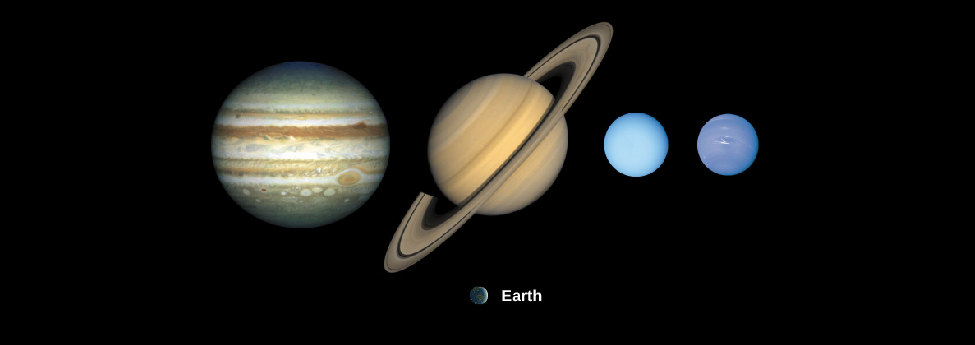
\includegraphics[width=3in]{Figures/Figure7.5.jpg}
    \captionof*{figure}{\scriptsize Credit: modification of work by NASA, Solar System Exploration}
\end{minipage}
\vspace{1em}

\question
Which planet is shown in below?
\vspace{1em}

\begin{minipage}{0.3\textwidth}
    \centering
    \begin{choices}
    \correctchoice Jupiter 
    \choice 
    \choice 
    \choice 
    \end{choices}
\end{minipage}%
\begin{minipage}{0.5\textwidth}
    \centering
    \begin{tikzpicture}
    \clip (0,0) circle (1.5cm);
    \node at (0,0) {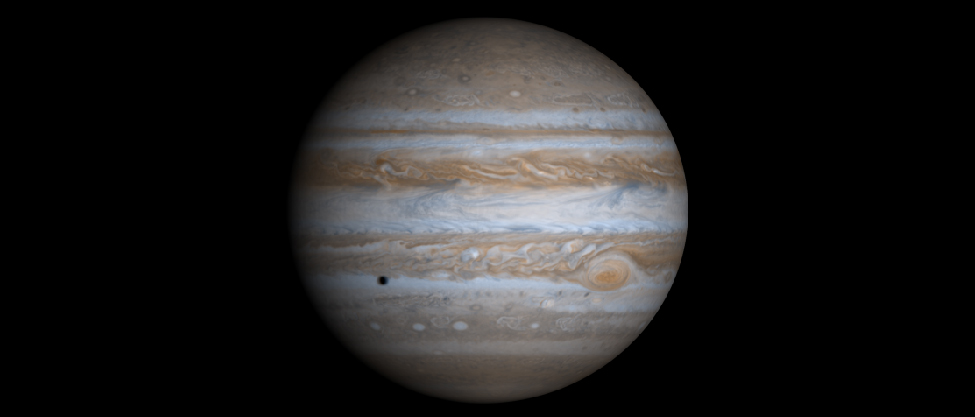
\includegraphics[width=0.5\textwidth,trim={1.5in 0 01.5in 0}, clip]{Figures/Figure7.11.jpg}};
    \end{tikzpicture}
    \captionof*{figure}{\scriptsize Credit: modification of work by NASA/JPL/University of Arizona}
\end{minipage}
\vspace{1em}

\question
Which object is shown in the image below?
\vspace{1em}

\begin{minipage}{0.3\textwidth}
    \centering
    \begin{choices}
    \choice the Moon
    \choice 
    \correctchoice Ganymede
    \choice 
    \end{choices}
\end{minipage}%
\begin{minipage}{0.5\textwidth}
    \centering
    \begin{tikzpicture}
    \clip (0,0) circle (1.35cm);
    \node at (0,0) {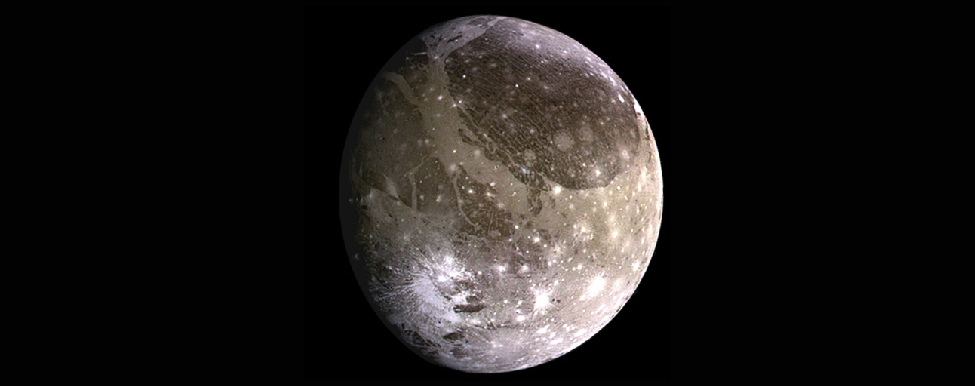
\includegraphics[width=0.5\textwidth,trim={1.5in 0 01.5in 0}, clip]{Figures/Figure7.12.jpg}};
    \end{tikzpicture}
    \captionof*{figure}{\scriptsize Credit: modification of work by NASA/JPL}
\end{minipage}
\vspace{1em}

\question
Ganymede is \fillin\ .

\begin{choices}
\choice the actual name of Earth's moon.
\choice 
\correctchoice one of Jupiter's moons.
\choice 
\end{choices}

\question
Which planet is shown in below?
\vspace{1em}

\begin{minipage}{0.3\textwidth}
    \centering
    \begin{choices}
    \correctchoice Earth 
    \choice 
    \choice 
    \choice 
    \end{choices}
\end{minipage}%
\begin{minipage}{0.5\textwidth}
    \centering
    \begin{tikzpicture}
    \clip (0,0) circle (1.6cm);
    \node at (0,0) {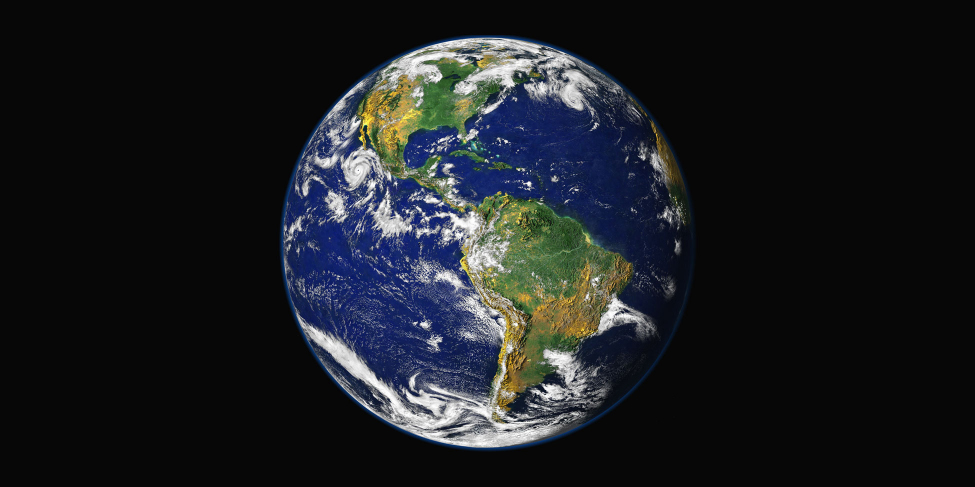
\includegraphics[width=0.5\textwidth,trim={1.5in 0 01.5in 0}, clip]{Figures/Figure1.6.jpg}};
    \end{tikzpicture}
    \captionof*{figure}{\scriptsize Credit: modification of work by R. Stockli, A. Nelson, F. Hasler, NASA/GSFC/NOAA/USGS)}
\end{minipage}
\vspace{1em}

\question
Which object is shown in the image below?
\vspace{1em}

\begin{minipage}{0.3\textwidth}
    \centering
    \begin{choices}
    \choice
    \correctchoice Pluto
    \choice
    \choice 
    \end{choices}
\end{minipage}%
\begin{minipage}{0.5\textwidth}
    \centering
    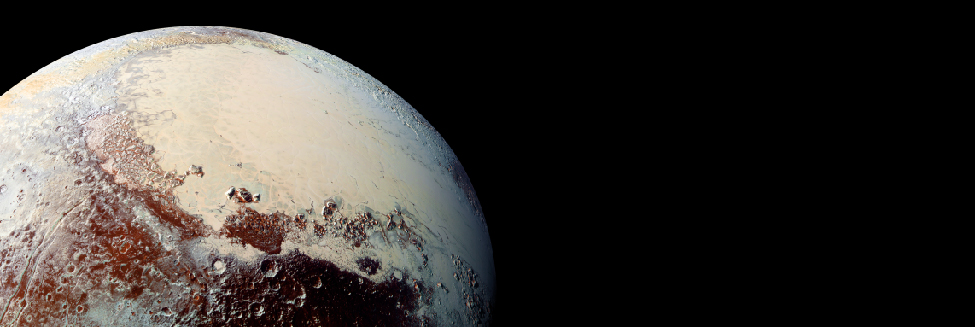
\includegraphics[width=0.5\textwidth,trim={0 0 2in 0}, clip]{Figures/Figure7.6.jpg}
    \captionof*{figure}{\scriptsize Credit: modification of work by NASA/Johns Hopkins University Applied Physics Laboratory/Southwest Research Institute)}
\end{minipage}
\vspace{1em}





\end{questions}
\end{document}